
\documentclass[runningheads,a4paper]{llncs}

\usepackage{amssymb}
%\setcounter{tocdepth}{3}
\usepackage{graphicx}

\usepackage{url}
\urldef{\mailsa}\path|{jharri1}@gmu.edu|
\newcommand{\keywords}[1]{\par\addvspace\baselineskip
\noindent\keywordname\enspace\ignorespaces#1}

\usepackage[caption=false]{subfig}
\usepackage{wrapfig}
%\usepackage{multicol}
\usepackage{amsmath}
\usepackage{color}
\usepackage{xcolor}
\usepackage{listings}

\usepackage{caption}
\DeclareCaptionFont{white}{\color{white}}
\DeclareCaptionFormat{listing}{\colorbox{gray}{\parbox{\textwidth}{#1#2#3}}}
\captionsetup[lstlisting]{format=listing,labelfont=white,textfont=white}

\lstset{
	language=Java,
	basicstyle=\small\sffamily,
	tabsize=4,
	numbers=left,
}

\renewcommand{\topfraction}{0.85}
\renewcommand{\textfraction}{0.1}
\renewcommand{\floatpagefraction}{0.75}

\providecommand{\abs}[1]{\lvert#1\rvert}

\newcommand{\doctitle}[0]{Retirement Redux: A replication of Axtell's and Epstein's Retirment Age model}

\begin{document}
\title{\doctitle}
\author{Ernesto Carrella \\ Joseph F. Harrison}
\authorrunning{\doctitle}
\institute{George Mason University}

\toctitle{\doctitle}
\tocauthor{Authors' Instructions}
\maketitle

\section*{Abstract}
This is the Abstract
\section{Introduction}
\label{sec:intro}

We replicated Axtell's and Epstein's Retirement Age model\cite{axtell_coordination_2006}.

\section{Model Description}

The model simulates retirement decision of heterogeneous agents.
Agents differ one from the other in terms of their behavior rules, social network and death age.
Every year every agent decides whether to retire or keep working. 

There are three tipes of agents.
Random agents choose whether to retire or not by tossing a coin.
Rational agents always retire as soon as possible.
Imitators instead do what the majority of eligibles do in their social network.

The main feature of the model is the gradual emergence of retirement norms.
Although 65 is fixed to be the retirement age, the population decides to retire at that age only gradually.
This paper tries to model retirement decision without economic rationale.
Mimesis is all that matter.

\section{Replication}

\subsection{MASON}

We decided to replicate the model trough the MASON framework.
This allows for the use of premade structures when programming in Java.
We did not have, nor we should have had, access to the original code in C.
Replication would be invalidated if we used anything but the original paper.

This allowed for the highlighting of both some advantages and disadvantages of Java and MASON.
These should be weighted by the added difficulty of not using NETLOGO or other ABM-specific languages.
One should also keep in mind that the original paper was also object oriented.

The greatest advantage of using Java is the ability to use premade structures.
We used an \textit{ArrayList} to store Agent's networks.
This allows us to remove deceased friends and to modify the size of the network over time.
For this very simple model, everything else would have been an overkill.

Another great advantage of Java is the proliferance of other packages we can integrate to our model.
OpenCSV was used to output formatted data.
Network packages like JUNG would have had very little added value.
Again, the simplicity of the model didn't call for any addition.

One feature of MASON is the complete separation between the graphic and the model code.
We decided to put this to a test so that each team-mate would focus on only one side of the code.
This proved not very succesful.
The model-side had to be progressively modified so that it would update the graphics-side at critical times.
This is particularly troublesome given the fact that in this model the graphical side is ancilliary.

\subsection{Object Orientation}

Intuitively, agents in this model share many similiarities.
They age, they die, they are either allowed or not to retire.
They are heterogeneous both in their endowments and their behavior.

Code-wise their different endowments are their variables, their different behavior are their class structure.
We can take advantage of Java's OO paradigm.
The UML diagram in figure~\ref{UML} describes the approach taken.
Most of the behavior is recicled from the \textit{Agent} abstract class.
Each subclass then overrides only the code pertaining retirement decision.

\begin{figure}
 \begin{center}
  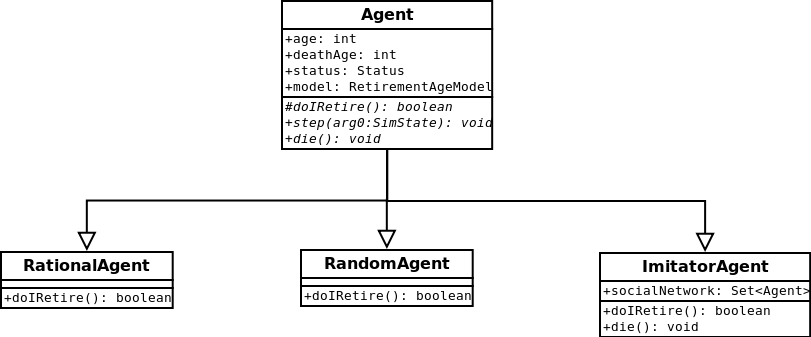
\includegraphics[scale=.45]{figs/UML.png}
\caption{The class structure of the agents}
\label{UML}
 \end{center}
\end{figure}



\subsection{Garbage Collection}

An important feature of Java is automatic garbage collection.
The programmer doesn't manually affect memory allocation. 
His responsibility is to remove any reference to the object he wants to delete.

Garbage collection proved quite a headache in our project.
All references to agents are stored in a single matrix.
We had hoped that by removing these agents from the matrix would be enough to clean the memory.
This proved unsuccesful.

One reason was MASON scheduler itself.
To run an agent in MASON one needs to schedule it.
Under the hood this means holding a reference of the agent in one \textit{heap} object, preventing garbage collection.
Scheduling comes into two types: scheduling once or scheduling forever.
Because our agents had to act every year, we scheduled them forever but that made their reference permanent in the heap.

This forced us into a ``least-worst'' analysis of our design choices.
We could schedule agents once every turn by checking if they were still alive.
This was bulky, burdensome and we would have had to create a new steppable just to make the check every turn.
Similiarly we could have made the matrix holding agents steppable and made it make checks and activate agents directly.
But with this we would have lost many advantages of the premade \textit{Schedule} class, in particular automatic shuffling of activation order.
The third way was to try and remove agents in the scheduler manually.

Stopping an agent scheduled forever proved more troublesome than it should be.
The \textit{Schedule} class does not allow for direct removal. 
The \textit{Steppable} interface, common to all agents, does not allow for stopping.
An unrelated \textit{Stoppable} is returned when the agent is first scheduled.
What we had to do was to manually store the reference to the stoppable and pass it to the agent after it has been scheduled.
Only then the agent dies can finally stop itself.

The other garbage collection issue was with social networks.
Agents every year purge their networks of their deceased friends. 
But when they ``die'' the remaining references in the \textit{ArrayList} are automatically not removed.
This meant that some of the old social networks referenced each other even when all its agents were dead.
This prevented them from being garbage-collected.




\section{Results}

%Interestingly, the age gap between new and old limit matters a lot!

\section{Discussion}
\section{Summary}

\bibliographystyle{splncs03}
\bibliography{references}

\end{document}
